
\chapter{商品检索与排序}

前文所述过程中建立的Lucene索引表和图像LSH哈希表是本章节商品检索与排序的根据,在本项目中,我们实现了两种检索方式——按关键词检索与按图片检索。

按关键词检索部分,用户可以输入商品关键词执行检索,也可以输入商品的品牌等属性执行高级检索。对检索的结果,用户可以选择按照相关度、价格顺序、评分高低进行排序。

在图片检索部分,用户上传图片后,可以选择LOGO匹配或精确匹配两种方式。\textbf{LOGO匹配}将图片与我们建立的产品品牌图库中的LOGO对比,计算SIFT特征向量的相似度,返回最有可能的品牌关键词执行关键词检索。\textbf{精确匹配}则将图片特征向量映射到前文建立的LSH哈希表中,返回匹配图片的URL列表,再到Lucene索引表中调用TermQuery匹配出URL对应的条目,按匹配度返回商品信息。

关键词检索与相关度排序沿用了本课程此前实验的代码,不作详述。本章节将主要介绍高级检索、商品排序和图片匹配三个功能的实现。

\section{商品高级检索}


\subsection{接口设计}

在此前建立索引的过程中,对于所有商品都具备的属性,如品牌、来源网站等,我们建立了专门的可被索引的Field进行存储,在本节我们将实现对这些Field的多字段检索。

在编写检索程序的代码前,考虑到我们的项目需要整合多种检索和排序方式,包括关键词、多字段检索、价格排序、评分排序等,我们有必要做好统一的接口,实现多重功能在后端查询时的一致。

一方面,用户可能在高级查询页面给出多字段的查询请求,对此我们采取了此前实验中类似的方法,编写了一个commandParser将查询条件转换成BooleanQuery处理多字段查询的请求。

尽管在查询首页中,用户输入的数据是以表单形式传入的,但我们在编写查询程序时,仍旧先将其转换成了一条“contents site:... brand:...”的字符串形式。之所以不直接提取表单内容而将其转换成字符串,是我们出于下文实现filter功能的考量,在filter功能中,用户在勾选过滤选项后会再次发出一个包含搜索的请求,网页需要保存记录此前搜索的字段传入filter请求的参数中,为了便于代码的复用,转换成字符串的方式会使程序更加可读和清晰。

另一方面,用户在结果页面可能会选择不同的检索方式,这会决定Lucene检索过程中searcher的参数,我们需要为此编写不同的搜索函数。在综合考虑整合以上两种因素后,以下是我们为检索程序提供的接口,可以看到,商品检索程序位于search\_command中,需要提供检索字符串kw和method(默认为按相关度relativity排序)两个参数。对获得的商品信息我们会做一些处理,获得filtertags等信息,具体将在前端部分进行介绍。

\begin{python}
# 统一处理搜索请求的web脚本 Web/code.py
class search:
    def GET(self):
        user_data = web.input(website="",brand="")
        kw = user_data.keyword
        if user_data.brand:
            kw += ' brand:%s' %(user_data.brand)
        if user_data.website:
            kw += ' website:%s' %(user_data.website)   # 将输入表单转换成字符串形式的请求
        method = web.input(method="relativity").method.decode('utf-8')
        vm_env.attachCurrentThread()
        contents = search_command(kw,method)     # 搜索结果
        filtertags = total(contents)           # 统计品牌、属性、特色的结果,即显示在页面左侧所必须的内容
        results = itemlis(contents)            # 要显示在页面右侧的所必需的内容
        return render.result(kw,method, results, filtertags)
\end{python}

\subsection{多字段查询处理}

在检索程序中,我们首先要对输入的query字符串进行处理,为此我们编写了一个command\_to\_query函数,统一处理各种形式的query。

\begin{python}
def command_to_query(command,analyzer):
    command_dict = parseCommand(command)          # 将字符串query转换成dict形式
    print command_dict
    seg_list = jieba.cut(command_dict['title'])
    command_dict['title'] = (" ".join(seg_list))  # 对command_dict遍历,建立BooleanQuery
    querys = BooleanQuery()
    for k,v in command_dict.iteritems():
        query = QueryParser(Version.LUCENE_CURRENT, k,
                            analyzer).parse(v)
        querys.add(query, BooleanClause.Occur.MUST)  # 各字段之间为AND关系
    return querys
\end{python}

对不同的检索方式,我们设计了如下结构以调用不同的搜索函数。
\begin{python}
def search_command(query,method):
    ... # 配置searcher、analyzer
    return globals()[method+'_search'](searcher,analyzer,query)
    # 根据method的不同调用不同函数名的搜索函数
\end{python}

至此,我们完成了搜索程序接口的设计,并且实现了商品的多字段高级搜索。

\section{商品按属性排序}

对具体的函数设计而言,我们有按相关度排序、按价格排序和按评分排序。相关度排序检测搜索结果与商品名称信息的匹配度,可以调用Lucene内置的scoreDocs方法实现,在此前的实验中已经完成,不作详述。对价格和评分排序,我们在建立索引时已经将这些信息用Lucene内置的LONG Field进行存储,我们只需为其建立对应的SortField,Lucene就可以实现按排序执行查找,以按评分查找为例,对应搜索程序的脚本如下所示。

\begin{python}
def rank_search(searcher, analyzer, command):
    rank_sorter = Sort(SortField("score",SortField.Type.LONG,True))  # True表明降序排序
    query = command_to_query(command,analyzer)
    scoreDocs = searcher.search(query, 150, rank_sorter).scoreDocs
    return read_results(scoreDocs,searcher) 
    # read_results函数提取搜索结果中的必要信息,将在前端部分介绍
\end{python}

\section{按图片检索}

\subsection{图片匹配}
根据我们已经建立的Hash表中包含了网页的URL和直方图特征向量。执行查询时,对输入的图片文件,我们计算图片文件的特征向量,将特征向量通过建表时相同的哈希函数映射到5张哈希表中,由LSH的局部敏感性质,我们认为哈希映射击中单元中的所有元素都和查询query具有一定的相似性。取5张哈希表中击中单元的并集,计算待查询的特征向量与我们存储的特征向量的相似度,就可以按序给出最接近的若干URL。

在查询的过程中,我们仅计算了5个哈希值,并仅对取出的n个元素(n远远小于数据集规模N)计算了匹配度,因此所消耗的时间是与数据集无关的常数时间。此外,由于我们的特征向量已经存放在了哈希表中,因此也可以保证计算匹配度的时间相较数据集规模N是常数的。该查询方式能够在时间上达到理想的效率。

\begin{python}
# 匹配图片函数
def match_pict(img):
    docs = []
    imgfeat = get_feature_Local(img)             # 计算查询图片的特征向量
    with open("hash_table.json",'r') as load_f:  # 打开本地哈希表文件
        load_list = json.load(load_f)
        for j in range(0,5):
            hash_val = LSHash(img,proj[j])       # 对查询图片进行哈希映射
            hits = load_list[int(hash_val)]      # 取出映射结果
            for hit in hits:
                elem = hit[0],similarity(imgfeat,hit[1])
                if elem not in hit:
                    hit.append(elem)             # 加入待排序集
    docs_sorted = sorted(docs,key = lambda kv:(kv[1]))
    res_lis = [i for (i,j) in docs_sorted[:50]]  # 取前50匹配的结果
    return res_lis                               # 返回50个最匹配的URL条目
\end{python}

\subsection{匹配条目查询}

上述过程中返回了一个URL列表,注意到URL是区分不同商品信息的标准,因此理论上有了URL就可以将搜索结果呈现在网页中。但不同于其他查询方式中返回包含所有信息的索引文档列表,在这里我们还需要对哈希表返回的URL列表元素在Lucene索引库中再查询,以获得商品的完整信息呈现在网页上,我们采用TermQuery的方式进行查询,如下所示。

\begin{python}
def pict_search(img):
    urls = match_pict(img)             # 调用上文match_pict函数执行LSH查询
    ... # 配置searcher,analyzer
    res_lis = []
    for url in urls:
        query = TermQuery(Term("url",url))   # 调用Lucene的TermQuery查询
        scoreDocs = searcher.search(query, 1).scoreDocs
        res_lis += read_results(scoreDocs,searcher)
    return res_lis                     # 返回的格式与其它查询函数接口一致
\end{python}


\part{Web Front-end}

\chapter{Web前端搭建}

在本项目中,前端的搭建基于web.py框架,在页面美化方面采用了Bootstrap框架。下面对Web前端的工作作具体介绍。

\section{web.py配置}

网站前端的URL结构如图\ref{fig:zlt_url}所示。

\begin{figure}[htbp]
\centering
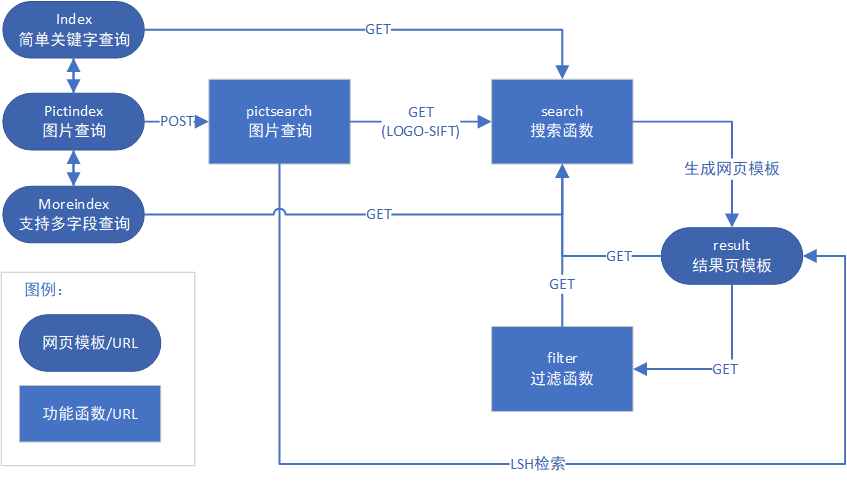
\includegraphics[width=13.5cm]{img/zlt/url.png}
\caption{网页URL组织形式}
\label{fig:zlt_url}
\end{figure}

在首页中,用户可以选择三种不同的搜索方式,对应三种表单,分别发起不同的request。简单的关键词搜索和支持多字段的高级检索会发起GET请求,将检索query传入上文构建的search函数。

上传图片的操作则会发起POST请求,POST请求首先将用户上传的文件保存到服务端,再根据用户选择的查询方式(LOGO匹配或精确匹配),调用对应的函数,返回响应的结果,处理POST请求的脚本如下所示。

\begin{python}
class pictsearch:
    def POST(self):
        x = web.input(input_img={})
        filedir = 'static/userupload'
        if 'input_img' in x:  # to check if the file-object is created
            fout = open(filedir + '/' + 'tmp', 'wb')
            # creates the file where the uploaded file should be stored
            fout.write(x.input_img.file.read())
            # writes the uploaded file to the newly created file.
            fout.close()  # closes the file, upload complete.
        # 将文件保存到本地
        if web.input().method == 'logo':
            kw = logo_recognition("static/userupload/tmp")  
            # 调用SIFT匹配函数,返回匹配的品牌关键词
            vm_env.attachCurrentThread()
            contents = search_command(kw,'rank'.decode('utf-8'))
            filtertags = total(contents)
            results = itemlis(contents)
            return render.result(kw, 'rank', results, filtertags)
        else:
            vm_env.attachCurrentThread()
            contents = pict_search("static/userupload/tmp")
            # 调用LSH检索函数,返回匹配列表
            filtertags = total(contents)
            results = itemlis(contents)
            return render.result('LSH Match', 'rank', results, filtertags)
\end{python}


无论是针对关键词还是图片的search函数,返回值均为一个包含所有检索匹配文档的列表,该列表会作为构造结果页模板的主要参数,决定结果页中的内容。结果页中也包含一个搜索表单和过滤选项,因此也可以发起搜索或过滤的GET请求,再次调用search或filter函数,刷新结果页的内容。


\section{搜索主页}

搜索主页如图\ref{fig:zlt_index1}、\ref{fig:zlt_index2}、\ref{fig:zlt_index3}所示。搜索主页包含了一个居中的表单。我们利用CSS样式表对页面进行了一些美化。如下所示的代码实现了背景图右下角的彩虹图案和搜索表单的半透明背景。

\begin{python}
/*** background picture ***/
body {
	background-color: rgb(0,0,0);
	background-image: url('../img/bg.jpg');
	background-repeat:no-repeat;
    background-position:bottom right;
	background-attachment:fixed
}
/*** index page ***/
#idx
{
	background-color: rgba(245,245,245,0.75);
	margin-top: 50px;
	padding-top: 50px;
	padding-bottom: 50px;
    text-align:center;
}
\end{python}

在本项目的前端实现中,我们还利用了Bootstrap的框架,该框架提供了良好的栅格排班系统和表单中需要用到的按钮等元件样式,极大提高了排版的效率和美观程度。我们在网页模板头文件中加入如下代码,即可在网页中调用Bootstrap框架预置的类样式了。

\begin{python}
<link href="https://cdn.jsdelivr.net/npm/bootstrap@3.3.7/dist/css/bootstrap.min.css" rel="stylesheet">
\end{python}

以单关键词检索表单为例,HTML代码如下所示。该表单会发起一个名为search的GET请求,传递的参数是一个名为keyword的字符串。

\begin{python}
# 单关键词检索表单示例
<form class="form-inline"action="/search" style="padding-bottom:10px " method="GET">
	<form class="form-inline">
	<input class="form-control"  style="width:40%"  type="text" id="keyword"
		   name="keyword" placeholder="Input Your Keyword"/>
	<button class="btn btn-default" id="Search" name="Search">搜索</button>
	</form>
</form>
\end{python}

最终搜索主页的效果如图\ref{fig:zlt_index1}、\ref{fig:zlt_index2}、\ref{fig:zlt_index3}所示。


\begin{figure}[htbp]
\centering
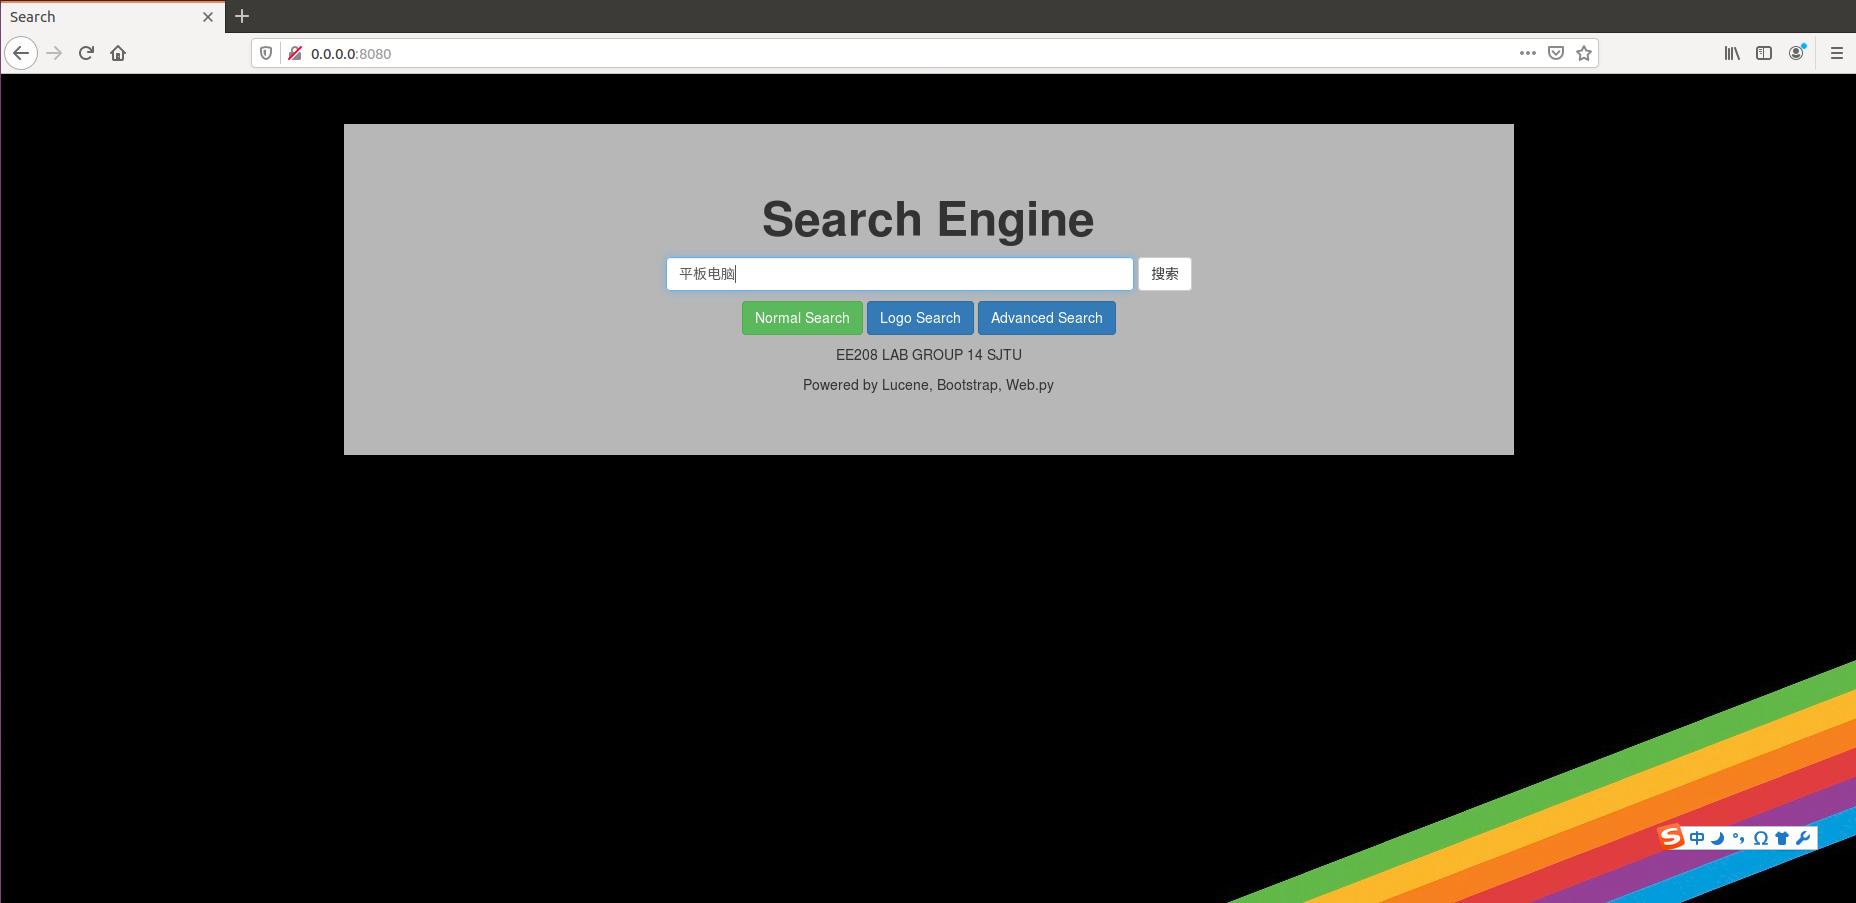
\includegraphics[width=9.5cm]{img/zlt/searchidx1.png}
\caption{单关键词查询首页}
\label{fig:zlt_index1}
\end{figure}

\begin{figure}[htbp]
\centering
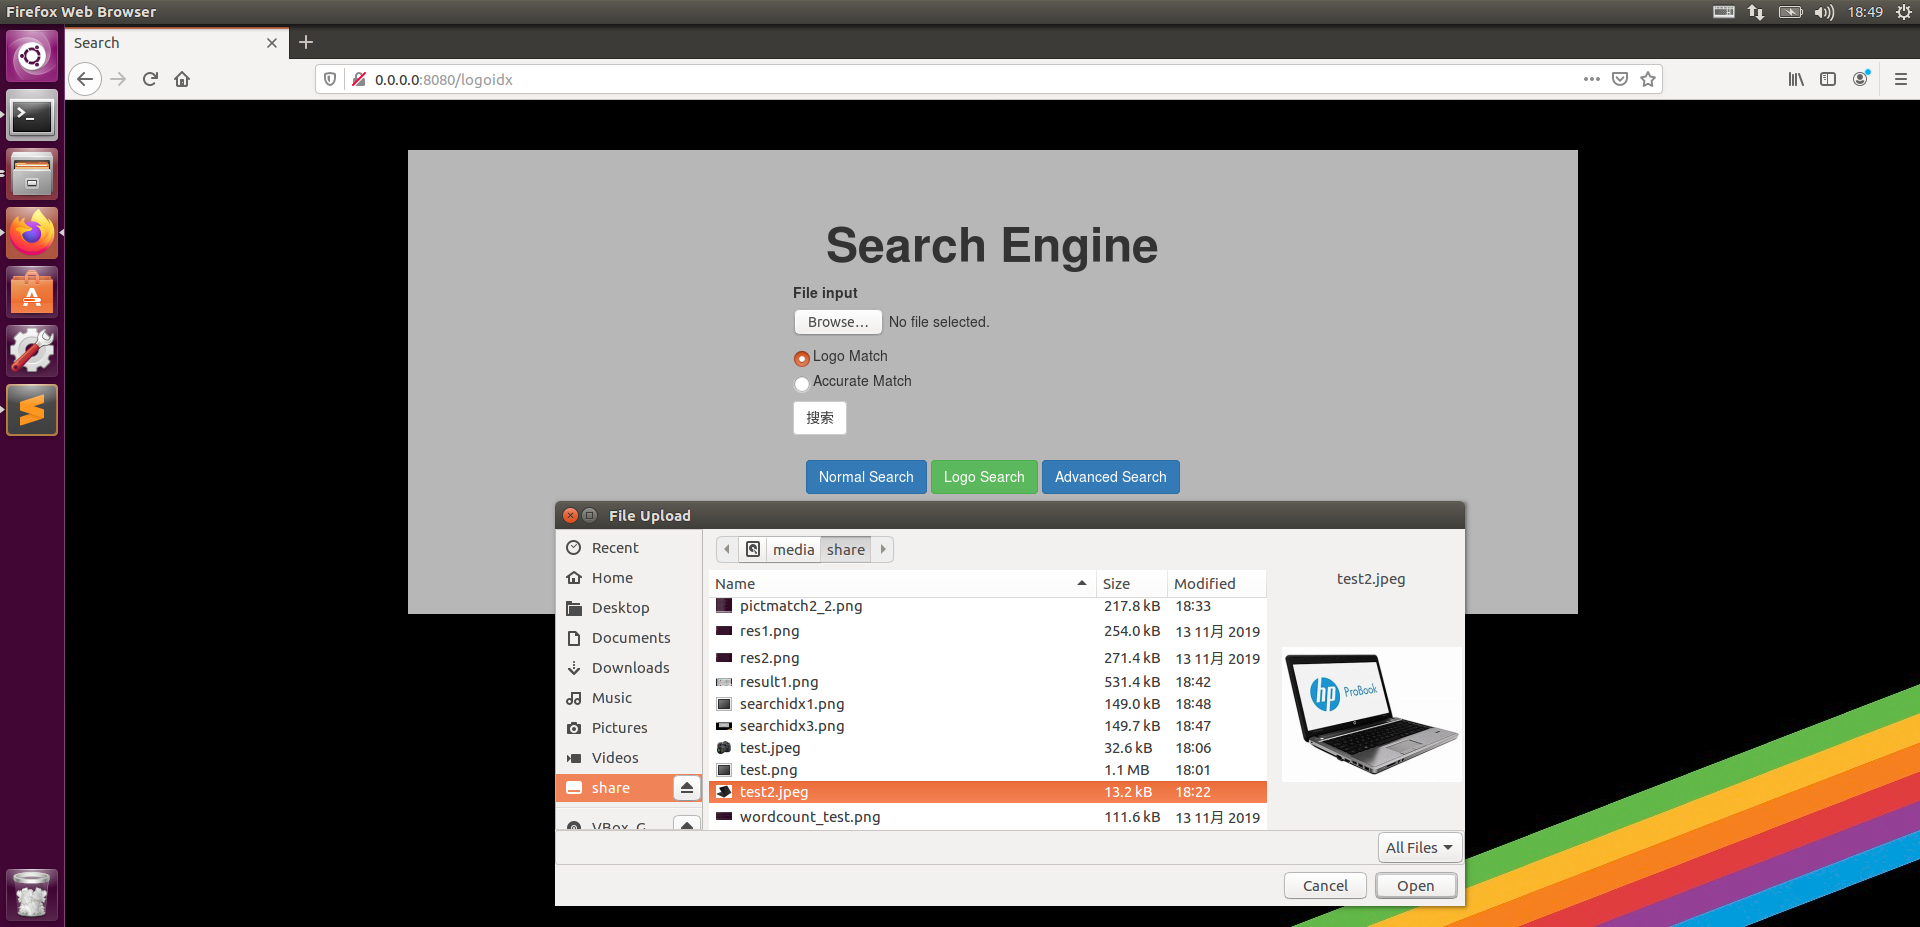
\includegraphics[width=9.5cm]{img/zlt/searchidx2.png}
\caption{图片查询首页}
\label{fig:zlt_index2}
\end{figure}

\begin{figure}[htbp]
\centering
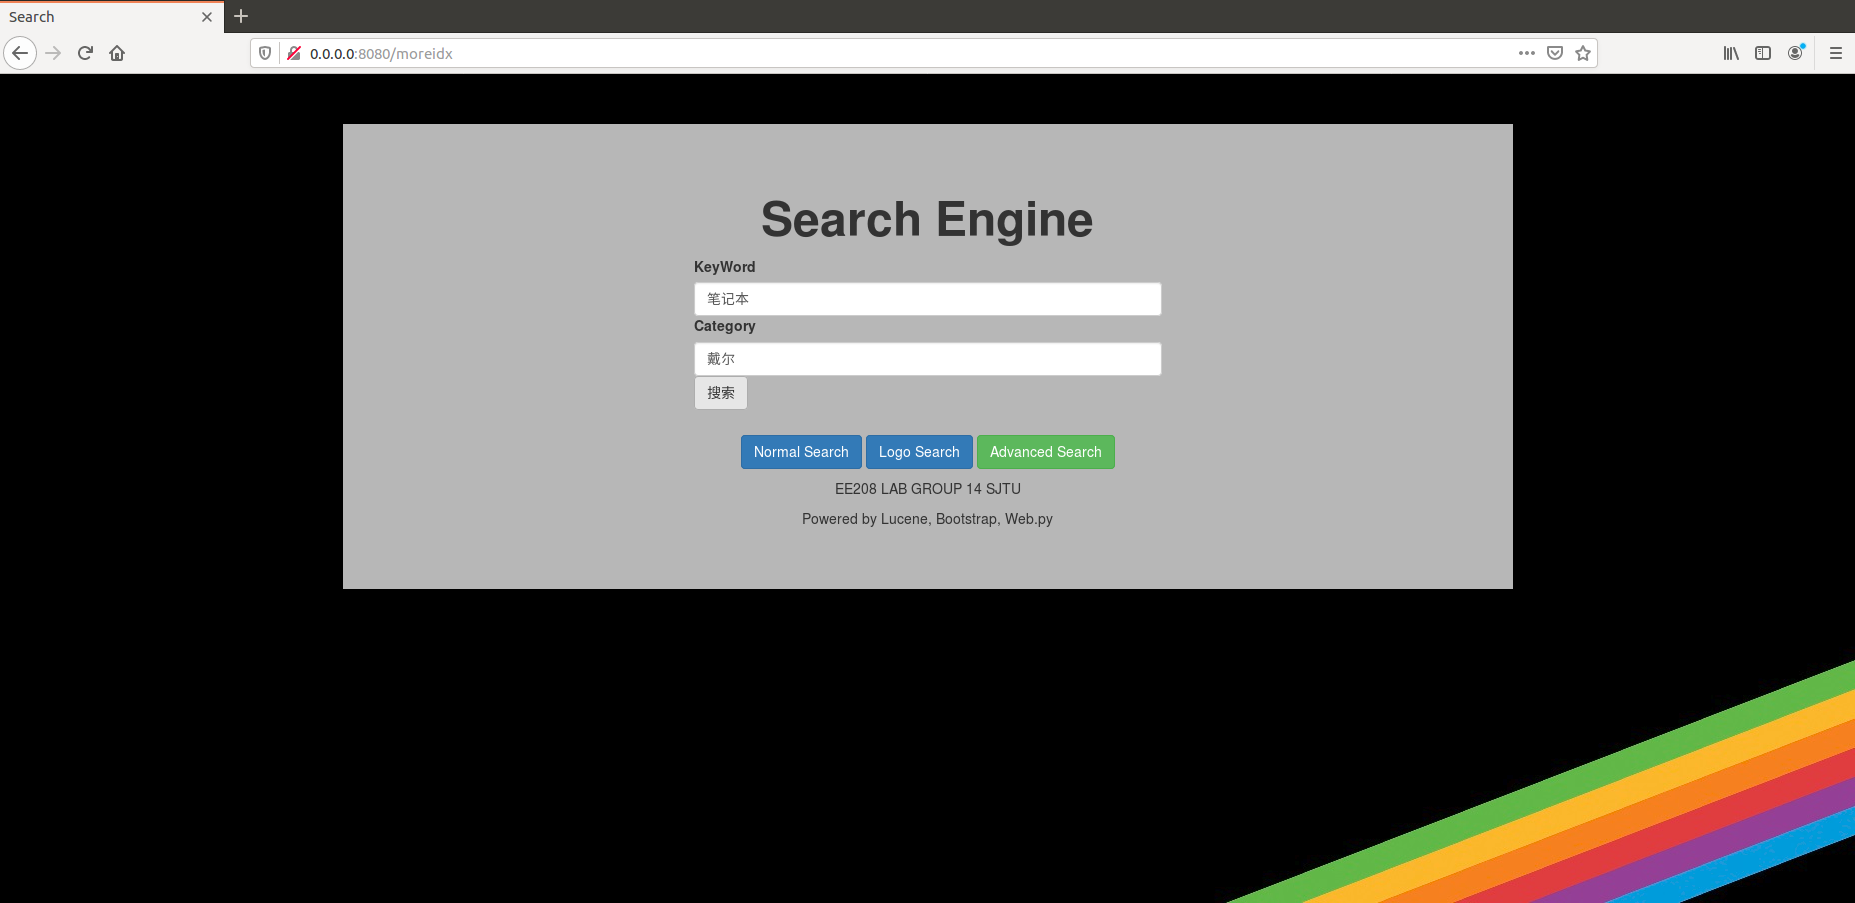
\includegraphics[width=9.5cm]{img/zlt/searchidx3.png}
\caption{多字段查询首页}
\label{fig:zlt_index3}
\end{figure}

\section{商品过滤功能}

我们的项目支持对搜索出来的结果进行过滤。过滤的对象包括商品品牌、商品类别、商品特征和商品来源。在大量商品的索引库中,直接统计所有商品的标签是难以实现的。因此,我们的解决方法是针对用户搜索返回的结果进行标签的统计和过滤。当用户发出search的请求后,网页在返回结果列表的同时,还会统计出结果商品的品牌、类别和特征,显示在网页的左侧,作为用户标签过滤的选项。

当用户在网页左侧的过滤中勾选了需要的选项,点击提交按钮后,网页会发出filter请求,网页将再次执行搜索,将搜索结果与用户勾选的选项匹配,在网页中返回筛选后的商品列表。下文我们将分节阐述该功能的具体实现。


\subsection{统计商品标签}

首先,针对search函数返回的商品列表,我们需要遍历contents列表,根据brand、category、feature等字段的组织形式统计所有可能出现的标签数,记录在一个dict中。随后,我们编写了一个sort\_and\_filter函数,对dict中的统计数从高到低排序。我们取排序前n个结果作为输出filtertags。这些选项将会出现在网页左侧供用户筛选。以下是sort\_and\_filter函数的脚本


\begin{python}
# 标签的统计与排序
def sort_and_filter(x_count,length):
    x_tuple = zip(x_count.keys(),x_count.values())
    x_sorted = sorted(x_tuple,key = lambda kv:(-kv[1], kv[0]))
    # 调用python内置的sorted方法对[(key,occurences)]列表进行排序
    filtered_x = x_sorted[:length]
    return filtered_x
\end{python}

以下是统计并返回tags的函数脚本,此处仅以brand为例。注意到实际中category、feature往往由多个字段组成,因此我们需要根据不同的字段采取不同的统计方法。

\begin{python}
def total(contents):
    # 返回三个参数的tuple,三个长度最长为n的[(key,num)]列表,分别是brand,category和feature的tag
    brand_count = dict()
    ...
    for item in contents:
        item = json.loads(item)
        brand = item['brand']
        ...
        if not brand_count.has_key(brand):
            brand_count[brand] = 0
        brand_count[brand] += 1
        ...
    # 以brand tags为例,统计过程如下。
    brand_tags = sort_and_filter(brand_count,5)
    category_tags = sort_and_filter(category_count,5)
    source_tags = sort_and_filter(source_count,2)
    feature_tags = sort_and_filter(feature_count,10)
    return [brand_tags,category_tags,feature_tags,source_tags]
\end{python}


\subsection{标签选项陈列}

根据上文返回的filtered\_tags,我们采取web.py中的for循环结构将标签作为表单的选项呈现在结果页左侧。对应的模板代码如下所示,我们仍然以brand为例。

\begin{python}
<h4 class="filter-title">品牌</h4>
$ count = 0
$for branditem in filtertags[0]:
    <label class="checkbox">
        <input type="checkbox" name="brand" id="brand$(count)" value="$(branditem[0])"> $(branditem[0])($(branditem[1]))
    </label>
    $ count += 1
\end{python}

\subsection{标签过滤请求}

用户在页面左侧勾选需要的选项后,表单将会发出名为filter的GET请求。web.py对该请求的处理过程如下所示。


\begin{python}
class filter:
    def GET(self):
        user_data = web.input()
        kw = user_data.keyword
        method = web.input(method="relativity").method.decode('utf-8')
        category = web.input(category=[]).category
        ... # 获取表单信息
        vm_env.attachCurrentThread()
        contents = search_command(kw,method) # 搜索结果
        filtertags = total(contents) # 统计品牌、属性、特色的结果,即显示在页面左侧所必须的内容
        filtered_contents = tag_filter(contents,category,features,brand,source)
                                     # 对搜索结果作筛选
        results = itemlis(filtered_contents) # 根据筛选结果提取出要显示在页面右侧的所必需的内容
        return render.result(kw, method, results, filtertags)
\end{python}

在tag\_filter函数中,我们会对Lucene的检索结果contents进行遍历,匹配返回符合用户输入的条目。

\begin{python}
# 商品与给定标签的匹配
def match_item(item,categorys,features,brands,sources):
    if not match_item_one(item,categorys,'category'):
        return False
    if not match_item_feature(item,features,'feature'):
        return False
    if not match_item_one(item,brands,'brand'):
        return False
    if not match_item_one(item,sources,'source'):
        return False
    return True

def match_item_feature(item,properties,property_name):
    # 与其他属性不同,特色取交集
    if (not properties):
        return True
    for proper in properties:
        if proper not in item[property_name].keys():
            return False
    return True

def match_item_one(item,properties,property_name):
    if (not properties):
        return True
    for proper in properties:
        if proper == item[property_name]:
            return True
    return False
\end{python}





\section{商品信息陈列}

\begin{python}
# 网页模板参数
def with (kw,method,contents,filtertags)
\end{python}

\begin{python}
# 读取商品信息
def read_results(scoreDocs, searcher):
    # 读取lucene检索结果对象ScoreDocs
    # 输出一个结果res_lis,list的元素是一个包含了商品所有信息的json串,在网页中可以用json.loads()解码
    res_lis = []
    for i, scoreDoc in enumerate(scoreDocs):
        doc = searcher.doc(scoreDoc.doc)
        item = dict()
        item['imgurl'] = doc.get("imgurl").strip()
        item['url'] = doc.get("url").strip()
        item['title'] = "".join(doc.get("title").split())
        item['brand'] = doc.get("brand")
        item['price'] = doc.get("price")
        item['rank'] = doc.get("score")
        item['category'] = doc.get("attribute")
        item['source'] = doc.get("website")

        # 商品具体属性
        itemdet = dict()
        detseg = doc.get("detail").split('\t')
        for detail in detseg:
            detailseg = detail.split(':')
            if len(detail)>1:
                itemdet[detailseg[0]]=detailseg[1]
        item['detail'] = itemdet

        # 商品评价tag
        itemfeat = dict()
        featseg = re.split(' ',doc.get("tag"))
        for feat in featseg:
            featureseg = feat.split('\t')
            if (len(featureseg)>1):
                itemfeat[featureseg[0].strip()]=featureseg[1]
        item['feature'] = itemfeat
        res_lis.append(json.dumps(item))
    return res_lis
\end{python}



\begin{python}
# 陈列商品信息
$def showdetails(details):
	<dl class="dl-horizontal">
	$for detail in (details):
		<dt>$(detail)</dt><dd>$(details[detail])</dd>
	</dl>
$def showfeatures(features):
	$for feature in (features):
		<button type="button" class="btn btn-default btn-sm">$(feature) ($(features[feature]))</button>
\end{python}

\begin{python}
<div class='result_contents'>
		$ count = 0
		$ pagecount = 0
		$for item in contents:
			$ count += 1
			$if (count%10 == 1):
				$ pagecount += 1
				<div id='page$(pagecount)' style="display: none;">
			<div class='row'>
				<div class='res' id='res$(count)'>
					<div class='col-md-3'>
						<a class='thumbnail' href='$(item["url"])'>
							<img class='img-responsive' src='$(item["imgurl"])' alt='$(item["title"])'>
						</a>
					</div>
					<div class='col-md-9'>
						<div class='row'>
							<a class="thumbnail" href='$(item["url"])'>
							<h3 style="width: 90%;overflow: hidden;white-space: nowrap;text-overflow: ellipsis;">
								$(item["title"])
							</h3>
							</a>
						</div>
						<div>
							<div class="col-md-4">
								<h4 class="price">¥ $("{:.2f}".format(int(item["price"])/100)) </h4>
								<p class="attributes"> $(item["category"]), $(item["brand"]), 评分 $(item["rank"])
								</p>
							<div>
								$:showfeatures((item["feature"]))
							</div>
							</div>
							<div class="col-md-8">
								$:showdetails((item["detail"]))
							</div>
						</div>
						
					</div>
				</div>
			</div>
			$:pageend1(count)
		$:pageend2(count)
	</div>
\end{python}

打印出了pageend的标签,这会在下一节介绍。

\section{翻页功能}

打印pageend标签,实现分区
\begin{python}
$def pageend1(count):
	$if (count%10 == 0):
		</div> <!-- end of page$(count/10)-->

$def pageend2(count):
	$if (count%10 != 0):
		</div> <!-- end of page$(count/10)-->
\end{python}

初始化

\begin{python}
<script type="text/javascript">
    function init() { 
		document.getElementById("page1").style.display="";
		document.getElementById("pg1").setAttribute("class","active");
    };
    init();
</script>
\end{python}

\begin{python}
# 按钮的JavaScript函数
var pages = $(pagecount);
function start()
{
	var pages = $(pagecount);
	document.getElementById("page1").style.display="";
	for (var it=2;it<=pages;++it)
	{
		var itit="page"+it.toString();
		document.getElementById(itit).style.display="none";
		document.getElementById("pg"+it.toString()).setAttribute("class","");
	}
	document.getElementById("pg1").setAttribute("class","active");
}
function end()
{
	var pages = $(pagecount);
	for (var it=1;it<pages;++it)
	{
		var itit="page"+it.toString();
		document.getElementById(itit).style.display="none";
		document.getElementById("pg"+it.toString()).setAttribute("class","");
	}
	document.getElementById("page"+pages.toString()).style.display="";
	document.getElementById("pg"+pages.toString()).setAttribute("class","active");
}
$for i in range(pagecount):
	function pg$(i+1)()
	{
		var pages = $(pagecount);
		for (var it=1;it<=pages;++it){
			var itit="page"+it.toString();
			document.getElementById(itit).style.display="none";
			document.getElementById("pg"+it.toString()).setAttribute("class","");
		}
		document.getElementById("page$(i+1)").style.display="";
		document.getElementById("pg$(i+1)").setAttribute("class","active");
	}
\end{python}

\chapter{项目成果}

\section{单关键词检索效果}

\begin{figure}[htbp]
\centering
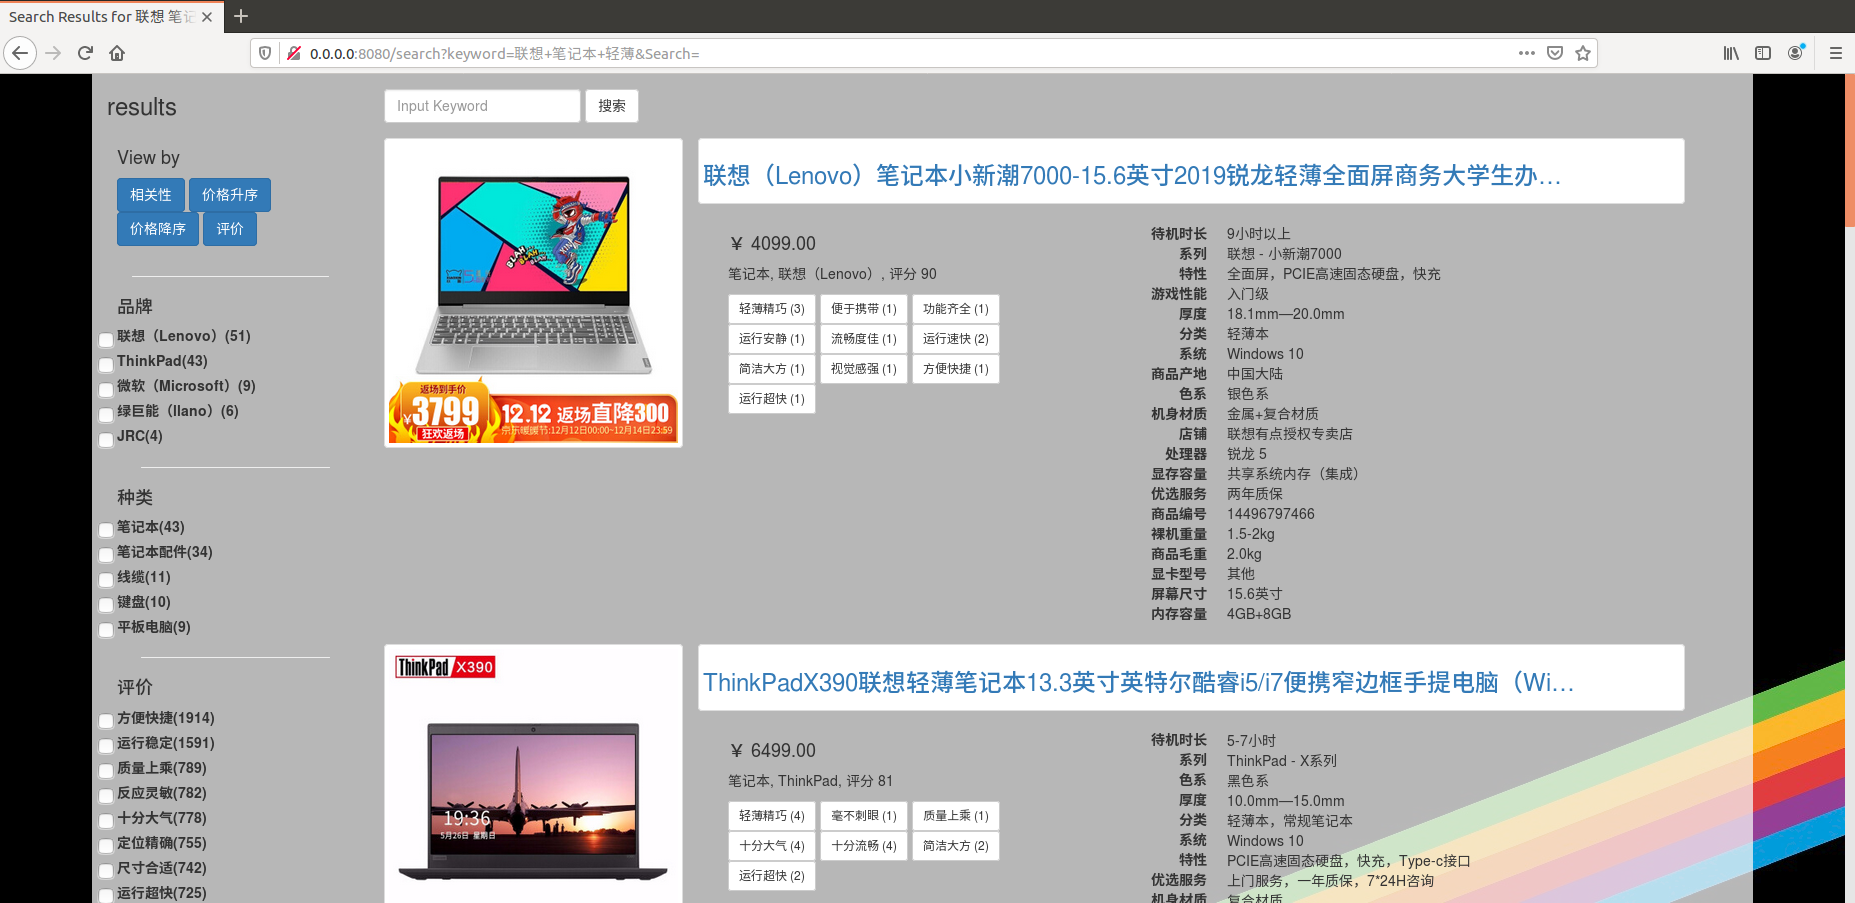
\includegraphics[width=13.5cm]{img/zlt/result1.png}
\caption{联想 笔记本 轻薄 为关键词的检索结果}
\label{fig:zlt_result1}
\end{figure}

\begin{figure}[htbp]
\centering
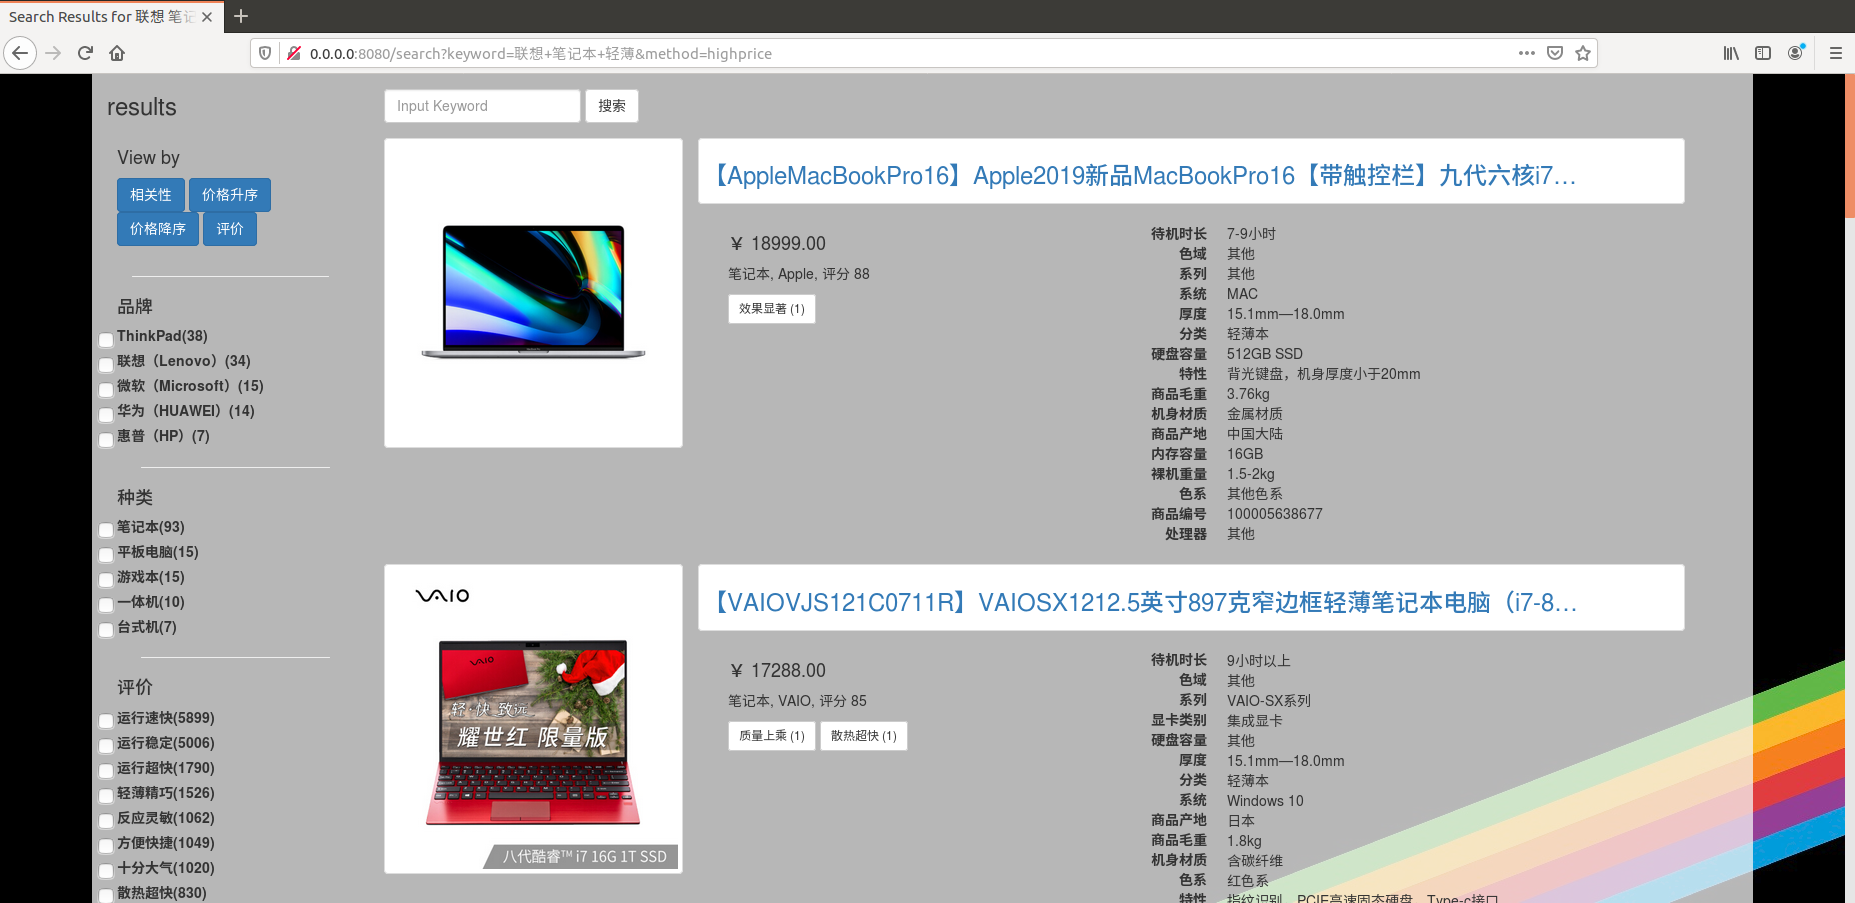
\includegraphics[width=13.5cm]{img/zlt/decreasing_price.png}
\caption{联想 笔记本 轻薄 为关键词的价格降序检索结果}
\label{fig:zlt_decreasing_price}
\end{figure}

\begin{figure}[htbp]
\centering
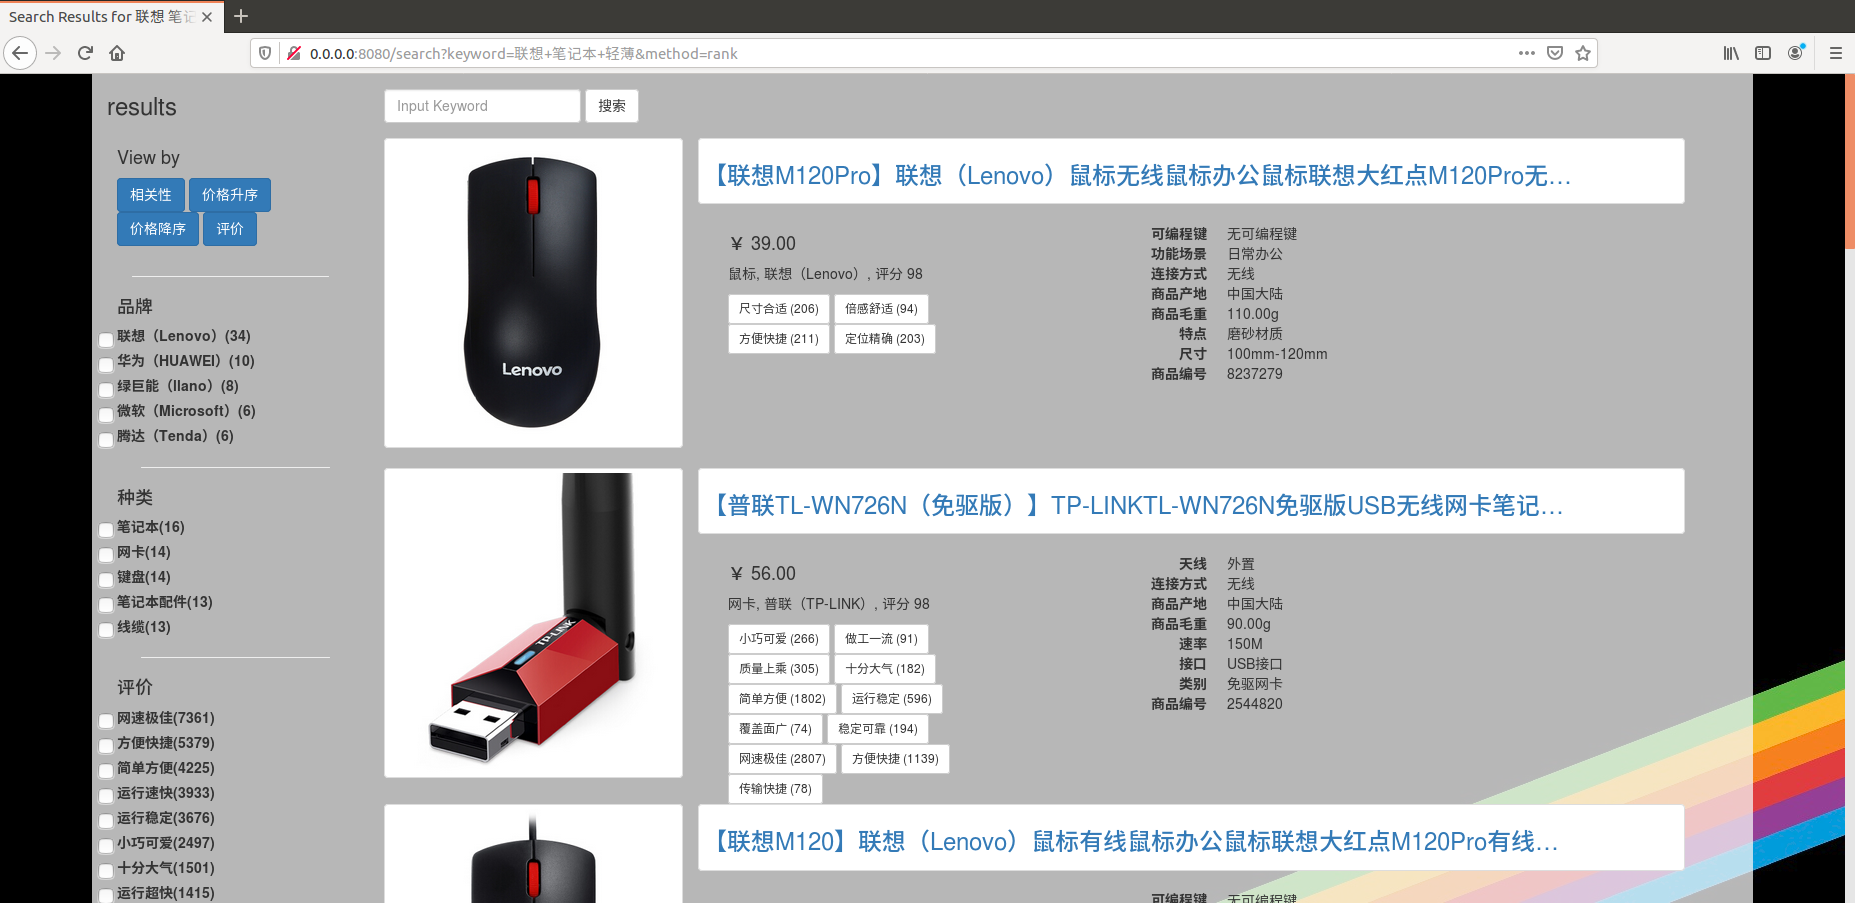
\includegraphics[width=13.5cm]{img/zlt/high_rank.png}
\caption{联想 笔记本 轻薄 为关键词的按评价排序检索结果}
\label{fig:zlt_high_rank}
\end{figure}

\begin{figure}[htbp]
\centering
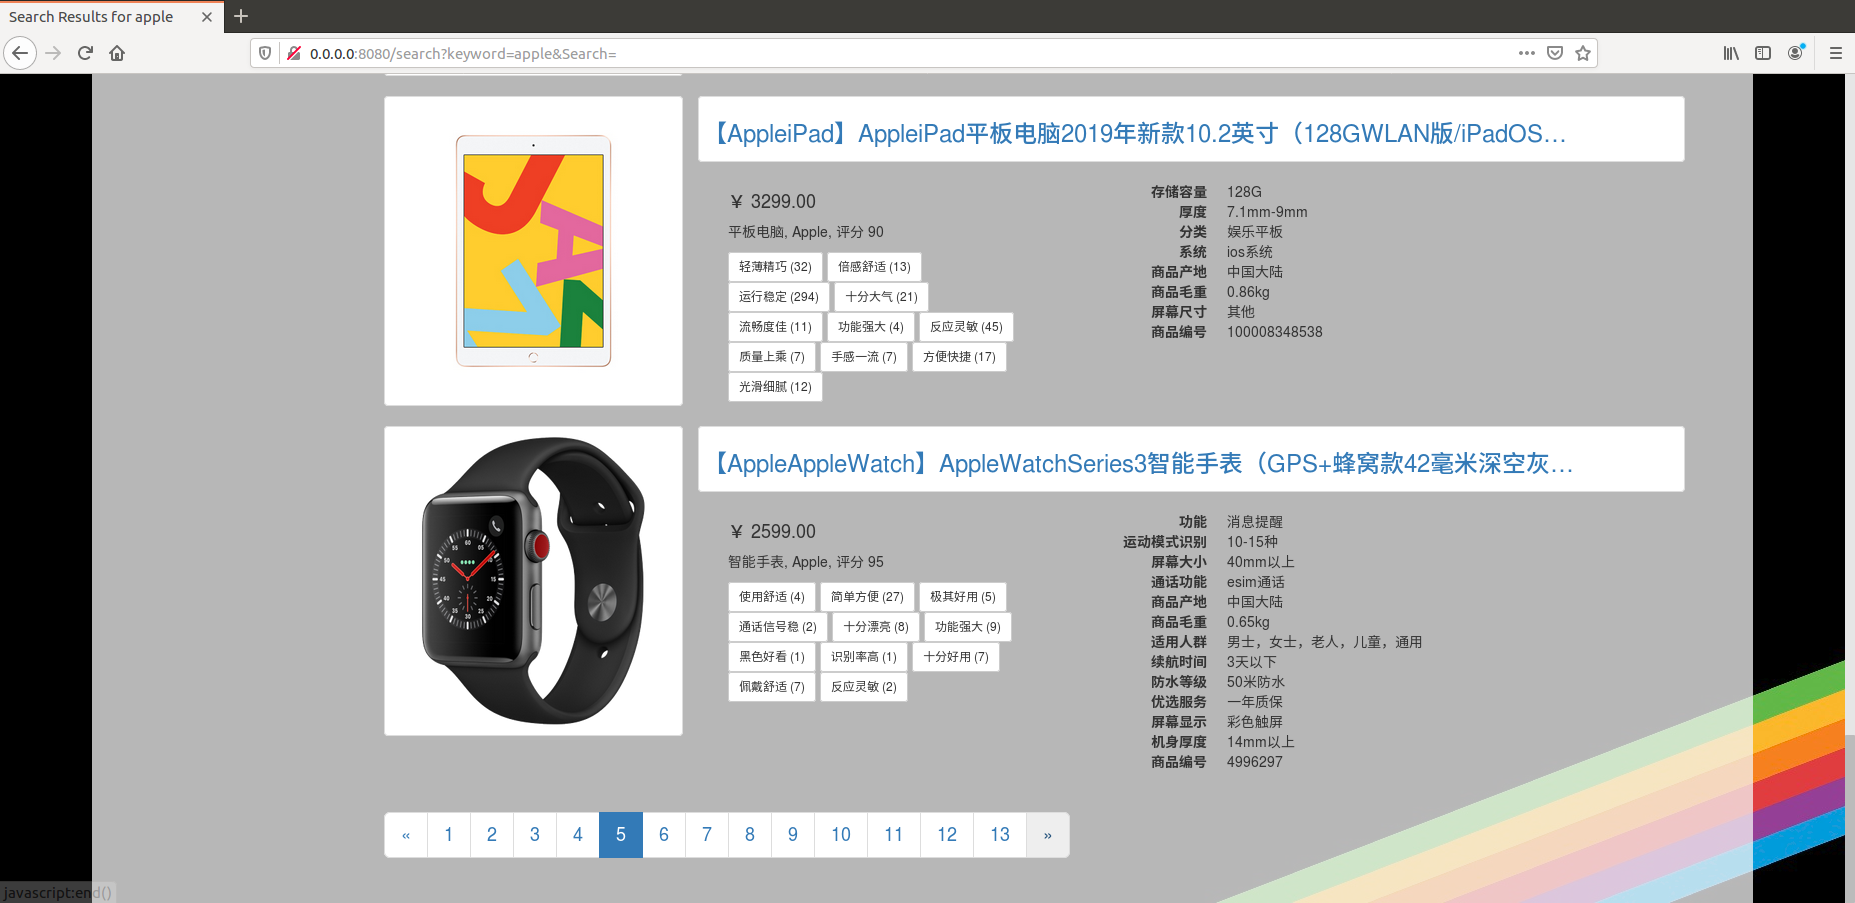
\includegraphics[width=13.5cm]{img/zlt/leafflip.png}
\caption{页面底部的翻页效果}
\label{fig:zlt_leaf_flip}
\end{figure}

\begin{figure}[htbp]
\centering
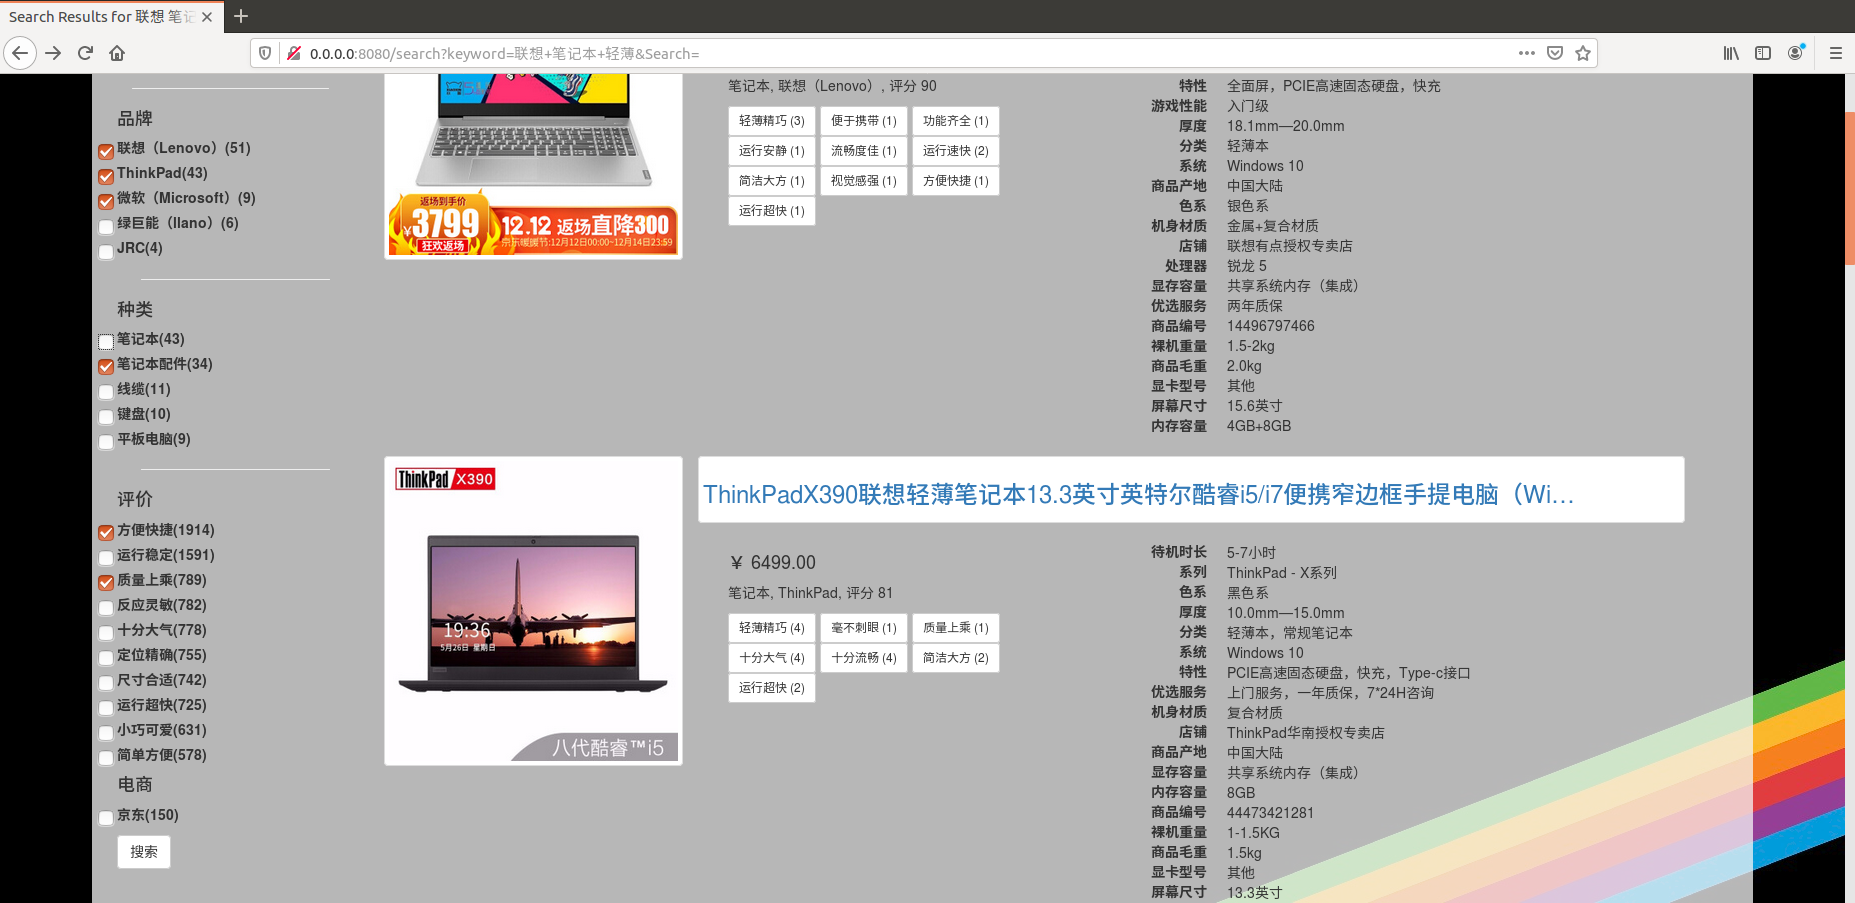
\includegraphics[width=13.5cm]{img/zlt/filter1.png}
\caption{结果过滤选项}
\label{fig:zlt_filter1}
\end{figure}

\begin{figure}[htbp]
\centering
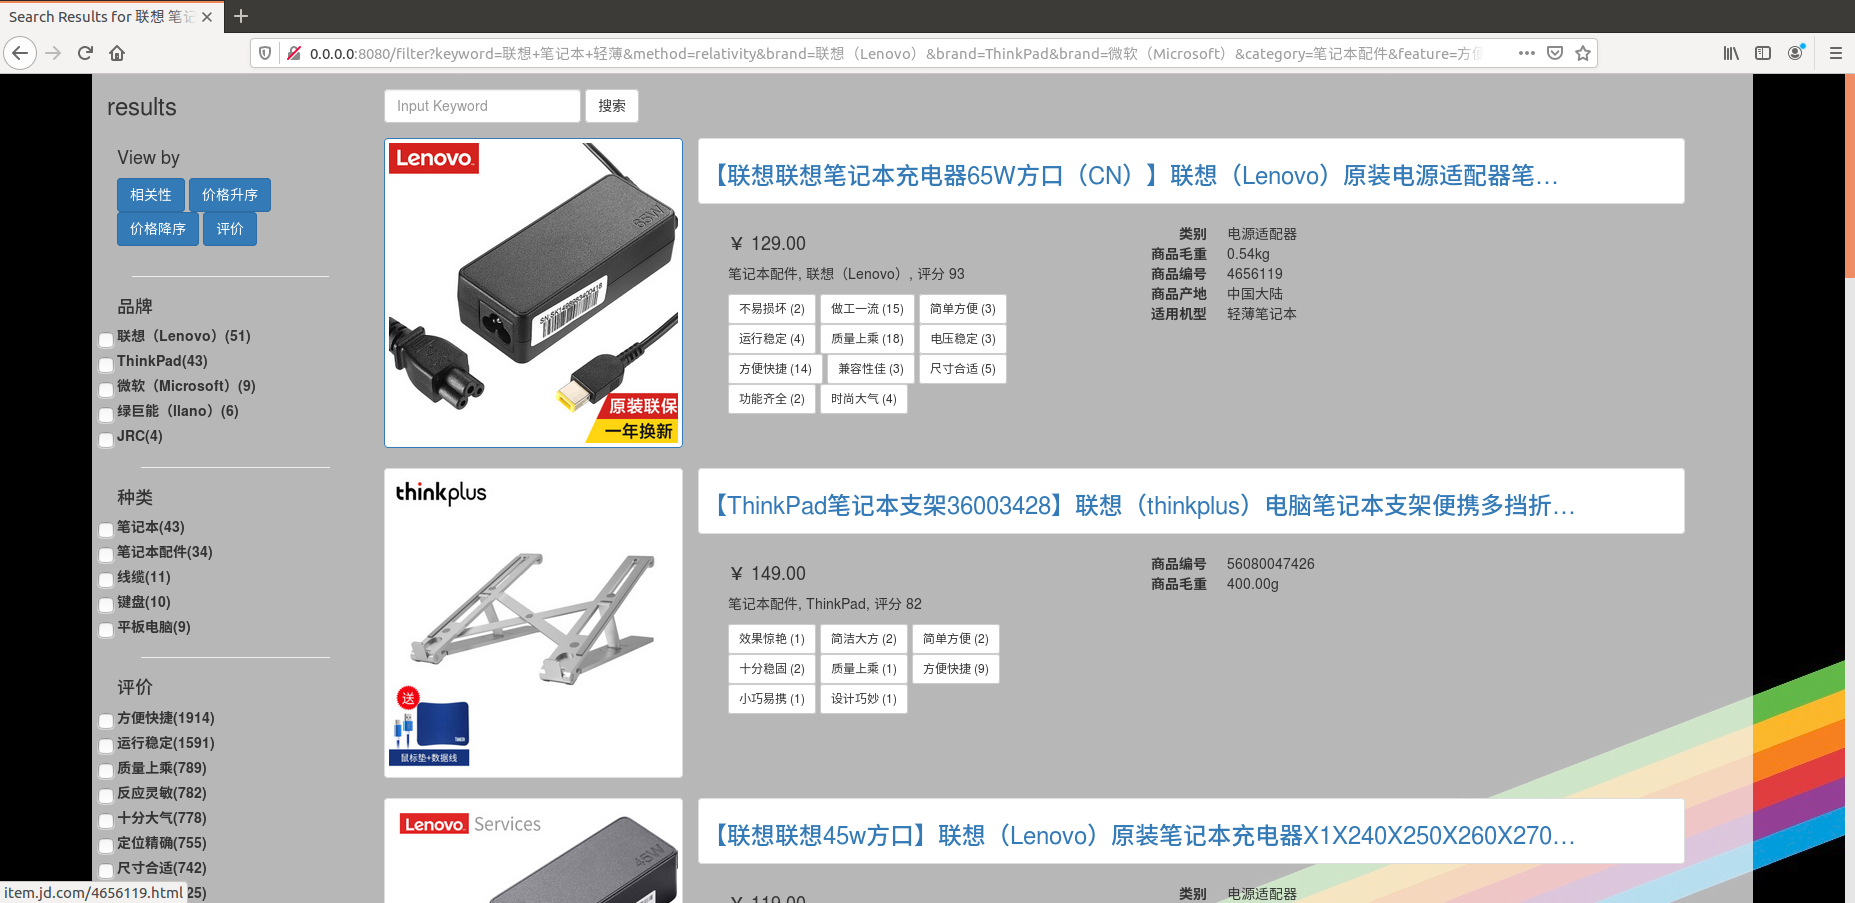
\includegraphics[width=13.5cm]{img/zlt/filter1_result.png}
\caption{过滤结果}
\label{fig:zlt_filter1_result}
\end{figure}

\section{logo匹配}

\section{图片LSH匹配}
